%-----------------------------------LICENSE------------------------------------%
%   This file is part of tikz_figures.                                         %
%                                                                              %
%   tikz_figures is free software: you can redistribute it and/or              %
%   modify it it under the terms of the GNU General Public License as          %
%   published by the Free Software Foundation, either version 3 of the         %
%   License, or (at your option) any later version.                            %
%                                                                              %
%   tikz_figures is distributed in the hope that it will be useful,            %
%   but WITHOUT ANY WARRANTY; without even the implied warranty of             %
%   MERCHANTABILITY or FITNESS FOR A PARTICULAR PURPOSE.  See the              %
%   GNU General Public License for more details.                               %
%                                                                              %
%   You should have received a copy of the GNU General Public License along    %
%   with tikz_figures.  If not, see <https://www.gnu.org/licenses/>.           %
%------------------------------------------------------------------------------%

% Use the standalone class for displaying the tikz image on a small PDF.
\documentclass[crop, tikz]{standalone}

% Import the tikz package to use for the drawing.
\usepackage{tikz}

% Tikz packages used.
\usetikzlibrary{arrows.meta, angles, quotes}

% Begin the document.
\begin{document}

    % Begin the drawing.
    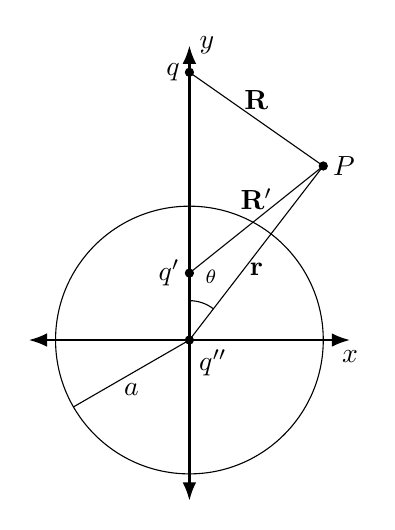
\begin{tikzpicture}[%
        > = Latex,
        scale = 1.7
    ]

        % Positions for all of the points.
        \coordinate (P) at (1.0, 1.3);
        \coordinate (q) at (0.0, 2.0);
        \coordinate (q1) at (0.0, 0.5);
        \coordinate (O) at (0.0, 0.0);
        \coordinate (a) at (-0.8667, -0.5);

        % Draw the coordinate axes.
        \draw[<->, thick] (-1.2, 0.0) to (1.2, 0) node [below] {$x$};
        \draw[<->, thick] (0, -1.2) to (0, 2.2) node [right] {$y$};

        % Circle about the origin.
        \draw (O) circle (1.0);

        % Connect the dots and label points and charges.
        \draw[fill, black] (O) circle (0.03) node [below right] {$q''$};
        \draw[fill, black] (P) circle (0.03) node [right] {$P$};
        \draw[fill, black] (q) circle (0.03) node [left] {$q$};
        \draw[fill, black] (q1) circle (0.03) node [left] {$q'$};

        % Draw and label the relative position vectors.
        \draw (O) to node [below] {$\mathbf{r}$} (P);
        \draw (P) to node [above] {$\mathbf{R}$} (q);
        \draw (q1) to node[above] {$\mathbf{R}'$} (P);
        \draw (O) to node [below] {$a$} (a);

        % Draw and label the angle theta.
        \pic[%
            draw = black,
            "\scriptsize{${\theta}$}",
            angle eccentricity = 1.7,
            angle radius = 0.5cm
        ] {angle = P--O--q};
    \end{tikzpicture}
\end{document}
